% Generated background with editable semantic labels; designed at 112 mm.
\begin{tikzpicture}[
  x=\linewidth,y=\linewidth,
  font=\figurefont\fontsize{8}{10}\selectfont,
  label/.style={draw=BookInk,fill=white,fill opacity=.92,
    text opacity=1,line width=.7pt,align=center,inner sep=1.5mm},
  action/.style={-{Latex[length=2mm,width=1.4mm]},
    draw=BookAmber,line width=1.2pt,rounded corners=1.2mm},
  feedback/.style={-{Latex[length=2mm,width=1.4mm]},
    draw=BookTeal,line width=1.2pt,rounded corners=1.2mm}
]
  \node[anchor=south west,inner sep=0] (scene) at (0,0)
    {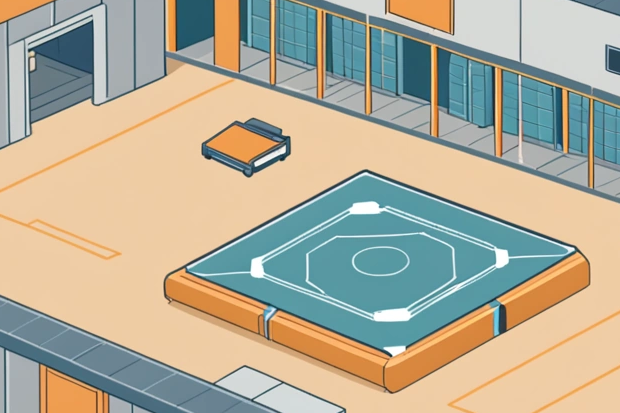
\includegraphics[width=\linewidth]{figures/rl-overview-embodied-setting.png}};

  \node[label] (agent) at (.19,.45)
    {\textbf{智能体}\\移动机器人};
  \node[label] (environment) at (.80,.45)
    {\textbf{环境}\\场地、障碍与目标};

  \draw[action] (agent.south) -- (.19,.08) -- (.80,.08)
    -- node[pos=.58,below,fill=white,inner sep=.8mm,text=BookAmber]
      {动作$a_t$：前进或转向}
    (environment.south);
  \draw[feedback] (environment.north) -- (.80,.62) -- (.19,.62)
    -- node[pos=.52,above,fill=white,inner sep=.8mm,text=BookTeal]
      {奖励$r_t$与下一状态$s_{t+1}$}
    (agent.north);
\end{tikzpicture}
